\documentclass[journal,10pt,onecolumn,compsoc]{IEEEtran} \usepackage[margin=1.0in]{geometry} \usepackage{pdfpages}
\usepackage{minted}
\usepackage{caption,graphicx,float} 
\usepackage{listings}

\usepackage{verbatim}
\usepackage{url}
\usepackage{nameref}
\graphicspath{/graphics} \setlength{\parskip}{\baselineskip} \setlength\parindent{24pt}
\usepackage[english]{babel}
%\usepackage{fullpage}

\title{TensorFlow\texttrademark WYSIWYG GUI Winter Term Progress Report}
\author{Group 33: Connor Sedwick, Behnam Saeedi, Collin Dorsett}
\date{\today}
\begin{document}
\maketitle
\begin{centering}
Fall 2016
\begin{abstract}
The purpose of this document is to discuss and outline the progress made on the  TensorFlow\texttrademark WYSIWYG Graphical User Interface system. 
Included is a discussion of project goals, current status, obstacles, and an overall retrospective of the past six weeks.
\end{abstract}
\end{centering}
\newpage
\tableofcontents
\newpage
%------------------------------------------------------------------------------
\section{Behnam Saeedi}
\subsection{Purpose and Goals}
\noindent The purpose of this project is to create a WYSIWYG -or What You See Is What You Get- graphical user interface for Google’s tensor flow machine learning API.
The goal is to create an interface that simplifies the user interface by abstracting away the syntax of the tool allowing the user to focus on their application on a conceptual level.
Such an interface has potential applications in a wide variety of fields other than computer science and software engineering.
Mathematics, statistics, business analysis and even marketing are examples of industries and fields that can take advantage of such a tool for creating Artificial intelligence software.
In mathematics, such a tool could be used for creating mathematical models, in statistics, it could be used for creating prediction and probability applications and in marketing and business it could be used for stock market, or analysis of benefits and risks.
%------------------------------------------------------------------------------
\subsection{Current State of the Project}
Currently we are in the development phase of the project where the GUI, data blocks and the core code generator of the tool is being implemented. Each one of these sections has an important and specific task. The GUI’s task is to create the user end of our system and collect the necessary data for generating the actual python code. This task is important because the it will be collecting all the different elements needed for code generation directly from user. Furthermore, this portion abstracts away the code complexity of an AI system. We are focusing on a specific functionality of a GUI for our implementation. This style is called WYSIWYG (Short for what you see is what you get). This approach helps user to design and see the system and software from a high level abstract perspective. User can use this method to create a flowchart like design of the system and expect the code to perform base on that blueprint. Next important portion in our system design is the core. The core has the task of interpreting the available data into python executable code. This portion behaves similarly to a compiler consisting of parsers, checkers, scanners, etc. The importance of this portion of our software is because this portion generates the final results. Without this portion our tool will not be able to create the required final python code. Finally, the Block  portion is the intermediary part between the Graphical User Interface and core where it describes the data required by GUI to draw the blocks while it is providing the data for the core to generate code. At this point on the graphical user interface side, several basic functionalities have been created such as buttons, menus, background and drag functionality. On the functional part, blocks and channel classes are implemented. The task of blocks class is to store the data needed for GUI in a specialized object that could be used for both code generation and GUI display. Furthermore, the basic functionality of channels is also created. Each one of these classes are also supplied with their own test case that test every functionality of that module. The test cases are series of assignments and declarations followed by assertion on their values after calls to their methods. These test cases show if there are any irregularities with the provided data and the results. Then, the test case displays the test itself with the result of the test helping us to identify where the bug occurred. Please refer to the code section at the bottom of the document for example of our test case implementation.
%------------------------------------------------------------------------------
\subsubsection{What Needs To Be Done}
On The GUI side, several features need to be added. These features include the function items, list of items in the menus on start up and implementation of the buttons. On the core side, the actual functionality of the interpreter needs to be implemented. Furthermore, this portion needs to be mounted to be used by other components of our software. Furthermore, the blocks need to be used as the position and data reference in the graphical user interface. After creating the GUI’s skeleton, we need to be able to mount these modules on the project and start using them as the backbone of our GUI for objects and  their positions. Furthermore, the core needs to be advanced in order to provide the necessary data for the GUI when the GUI become partially functional. These parts perform the task of generating the list of methods required by the graphical user interface, generating the tables and tokens needed for interpretation of the GUI to python, check the semantics of the project and finally generating the python code. The tokens are listed in a table which has the task of tracking the priority and the use of each method call. This table is going to make it very easy to generate the required code.
%------------------------------------------------------------------------------
\subsection{Problems and Solutions}
Our project has faced several problems relating to our implementation and some of the APIs we have been using for the implementation of graphical user interface. It appears that the API which we selected for our GUI was not as flexible as we expected it to be. Furthermore, our API has a rich documentation for mobile devices but not on PC platforms. On the core portion of the project there have been complexions with the means of interpreting the data collected from graphical user interface to machine readable data. We are looking into possible solutions  to this problem. First step which we took was to re evaluate the priority of different portions of our development and increased the work force working on the graphical user interface portion of the code. Furthermore, we are planning to communicate more on the problems which show up on the GUI implementation to make it easier for every member to develop a solution. On the core side, flexible and adjustable placeholders are needed for an easier transition of data between the GUI and core. One of the setbacks which we faced was caused by bad implementation of the data token system. This portion underwent several important changes to match the clients requirement.
%------------------------------------------------------------------------------
\subsection{Experimental designs}
We had several experimental designs for this data token handling. These designs took advantage of a database system (MySQL in this case) for managing the tokens and their priority. This would have been a proof of concept for us to also use it for our save functionality. However, our stakeholder did not wanted our system to depend on an external database that might require a large amount of configuration and setup. This design was dropped and for the purpose of our project, we will be creating costume save objects to be loaded and unloaded on to and off of python. Based on the requirements by our stakeholder, there are no restrictions on the formatting of save data. We also started researching alternative graphical user interface development APIs in case the documentation for Kivy was not sufficient to satisfy our requirements for this project. On the core sides too we are looking for possible solutions to the complications we are facing. In the meantime, we are researching some of the most efficient designs which we can provide for the core portion of the WYSIWYG API. We are specifically looking into compiler designs available since our system behaves like a compiler converting a program in a source syntax (in this case a graphical representation) to the destination syntax (in this case python). It is important to not reinvent the wheel in this project especially since the time provided for developing this tool is not enough. 
%------------------------------------------------------------------------------
\subsection{User Studies}
We still haven’t preform our user experiments. However, we have closely looked into usability of our GUI after we created our mock-up. We are hoping to be able to create an alpha version of this tool running soon to be able to test and modify our design for making the tool more efficient and easier to use.
%------------------------------------------------------------------------------
\section{Connor Sedwick}
\subsection{Purpose and Goals}
\subsubsection{Purpose}
The main purpose of our project is to work closely with our stakeholder to research and develop a software that can aid in developing and visualizing deep learning algorithms.
We are also treating the project as a learning experience for best design practices.
\subsubsection{Goals}
Our goals for this term are to develop of our Graphical User-Interface and core algorithms for use in our project. 
One of our sub-goals is to be able to have our project tested during Winter term by our stakeholder's students to aid us in development.
To do so means we will likely be testing individual features of our software throughout development.
%------------------------------------------------------------------------------
\subsection{Current State of the Project}
As of Week 6 of Winter Term, we have an alpha release of our Graphical User-Interface to demo as well as some core software for the back-end of our project.
The Graphical User-Interface has a base layout containing buttons and a drag-able object with text input. 
We are currently working on changes to the Requirements document and possibly the Design document to remove a redundant feature that our stakeholder has pointed out to us.
We have decided on a tri-weekly meeting system with our stakeholder. 
This was decided at the beginning of the term.

\noindent Since our last meeting with our stakeholder we now realize that we need to shift focus more on developing the interface further in order to get it working well enough to test with our core code.
We need to be able to implement the core code for Blocks with the drag-able objects in our interface.
We are currently also working on developing a priority system for objects placed in our GUI that will aid our system with reading the user's Block placement and choices and translate it into the proper Python code.

\subsection{(Connor Sedwick) What Needs To Be Done:}
We need to get event-handling working properly with the interface to generate drag-able Block objects to the interface on a button push. 
We may need to research another toolkit for our interface.

\noindent We need to develop a testable prototype to demonstrate the object handling between the Block objects dragged onto the interface and the Block objects defined in the core code.

\noindent Our core code needs a priority system set in place to rank objects and aid in the generation of Python code from the text input embedded in our Block objects.

\noindent We also need to set up a comment Block item for our GUI that allows users to create notes for their code.

\noindent On the whole, we need to get a connection going between the core classes and the objects appearing in our GUI. 
Currently, there is no clear connection between the core and GUI. 
This could be done with simple test cases where a Kivy object and one of our core Block objects are implemented together.
%------------------------------------------------------------------------------
\subsection{Problems and Solutions}
\subsubsection{GUI}
Being new to UI design I spent much time viewing the documentation and watching tutorials for the Kivy API.
Kivy uses ".kv" files which act similarly to Cascading Style-sheets in HTML.
At first the work was very intuitive and I was able to easily put together a base layout for our GUI.
The tutorials online were very informative at first with how to format ".kv" files to get the layout I desired.
As I moved onto adding buttons and working with events I found myself in a bit of a snag.
Tutorials on drop-down menus with Kivy are very sparse and I had to spend much time trying to figure out how drop-downs worked due to the lacking documentation the Kivy website offered.
Eventually, I was able to piece together how to handle drop-down events after referencing some open-source code and forum pages.
It turned out that the drop-down object must be called with a "dropdown.open()" function from the button attribute "on\_release:".

\noindent With the drop-down functionality for our menus figured out, I turned to working on getting our drag and drop features implemented.
Again, the Kivy website had sparse documentation on drag-able objects.
I was able to refer to a Kivy demo code a few times in order to understand the functionality of dragging object around a screen.
The issue I ran into soon after was with trying to generate drag-able objects at the push of a button.
This led me to read up more on syntax with object definitions, file importation, and how objects of different classes interact in Python.
As a result, I often found myself having to reformat my files numerous times.
What I believe I need to do to fix this issue is to develop and define individual classes in our main Python file which controls the GUI.

\noindent Another issue I have run into with the Kivy API is that it does not appear to support vector graphics. 
This is troublesome because we are trying to implement icon buttons in parts of our GUI.
The current icons that we are using do not appear correctly within the buttons on the GUI as a result of this. 
This has led us to deliberate on whether we want to stick to text buttons.
\subsubsection{Meeting times}
We have had some issues with meeting as a team this term. 
Because our schedules are so mixed it is difficult to group together to work on specific features as a team. 
We have been making extensive use of email and online chat rooms to discuss our project and work on it.
Lately, I have been dropping into Behnam's office to check-in on his progress with the core and bring him up to speed on the current state of the GUI. 
Collin's schedule appears to have been very busy and he has had trouble meeting with us to discuss work.

%------------------------------------------------------------------------------

\subsection{Retrospective}

\begin{table}[H]
\begin{center}
 \begin{tabular}{ |p{0.3\textwidth-2\tabcolsep}|p{0.3\textwidth-2\tabcolsep}|p{0.3\textwidth-2\tabcolsep}|} 
 \hline
 \multicolumn{1}{|c|}{\textbf{Positives}} 
 & 
\multicolumn{1}{|c|}{\textbf{Deltas}}  & 
\multicolumn{1}{|c|}{\textbf{Actions}}\\
 \hline
 
Our open schedules allow us to drop in at Behnam's office and discuss work & Need to meet as a team rather than communicate online & Have talked with TA and are setting up meeting times for each week to hammer out the remaining parts of the project.\\
 \hline
 
Was able to quickly develop a window and layout for our GUI with our current toolkit & Documentation for specific functions and features is somewhat lacking &  Find tutorials and examples online of projects made with our current toolkit Kivy \newline May look into changing toolkit  \\
 \hline
 
Gleaned much information from weekly TA meetings by writing up talking points prior to meetings & & \\
 \hline
 
 \hline
\end{tabular}
\caption{A retrospective of the past six weeks.}
\label{table:1}
\end{center}
\end{table}

%------------------------------------------------------------------------------
\section{Collin Dorsett}
\subsection{Purpose and Goals}
\noindent The main purpose of our project is to work with our client to research and develop a software that can aid in developing and visualizing deep learning algorithms. We are also treating the project as a learning experience for best design practices. One of our major goals is to be able to have our project tested during Winter term by our client's students to aid us in development. To do so means we will likely be testing individual features of our software throughout development.
%------------------------------------------------------------------------------
\subsection{Current State of the Project}
\noindent As it stands, the GUI of our program is nearing completion. The layout of the program's GUI follows our initial design as presented in the design document. A comparison of the initial design and current layout are included in the 'Images' section. All items/buttons within the GUI are click-able; however, they have no functionality, as we are still working on the back end of the program. Additionally, we were able to include the ability to drag a test Block around the Scene area.\\\\
\noindent Regarding the back end of our program, most of the foundations are already in place. We did, however, run into some problems with the actual implementation of the back end (explained below). Once the GUI portion of the program is completed (or nearing completion), the back end will become the main focus of the project. This is because the back end will need to successfully pull data from the Scene area of the program in order to communicate with TensorFLow\texttrademark.
%------------------------------------------------------------------------------
\subsection{What Needs To Be Done}
\noindent Our main short term goal is to incorporate a drag-and-drop feature to the Block menu of the program. Ideally we will be able to drag various Blocks from the Block menu into the Scene area. Additionally we need to incorporate a way for the Blocks to be connected to each other via Channels. We also need to include to options to start a new project, save the current project, run the current project, stop the current project, or extract the current project. These particular commands will need to be implemented in the back end of the program.\\\\
\noindent Although we have a solid foundation for he back end of the program, we still need to spend some time developing the back end. Our main goal here will be to have the back end successfully communicate with TensorFlow\texttrademark. The next step will be to have the back end pull data from the Scene area and compile a list of commands to be sent to TensorFlow\texttrademark.\\\\
\indent Once we have finished most of our front and back end we plan on holding some user study sessions with the very students that we hope will be utilizing this program. From their feedback and testing we should be able to further fine-tune the program to their expectations.
%------------------------------------------------------------------------------
\subsection{Problems and Solutions}
\noindent One major problem that occurred was the ability to add a drag-and-drop feature to the program. Although this is one of the defining features to this program, it is quite difficult to successfully implement due to lack of online documentation for the Python module kivy. With this lack of information, much time has been spent on trying to figure out how to successfully implement this particular feature.\\\\
\noindent Another issue arose during the development of the back end of the program. Although not as detrimental as the previous issue, our group attempted to utilize SQL in order communicate with TensorFlow\texttrademark. However, after some discussion with our client, we came to the conclusion that this additional software would take away from our initial goal of keeping the program simple and easy to use. As such we are working on other methods of communication with TensorFlow\texttrademark.
%------------------------------------------------------------------------------
\subsection{Experimental Design} 
\noindent As mentioned previously, there were some issues that came up trying to implement the drag-and-drop feature. We have considered using a different Python module for development instead of kivy. One of the options we looked into was Mirra, a Python framework that utilizes 2D OpenGL, similar to kivy. This particular module focuses on user interaction and implements an event listener and classes that receive mouse events. While this would be a good fit for our project, we are still in debate over whether or not we should completely revamp our program.\\\\
\noindent Regarding another issue mentioned previously, there was some discussion about the actual implementation of the back end. Initially we had used SQL to communicate with TensorFlow\texttrademark, however, our client felt that this was an unnecessary addition to the project. After talking with our client we decided to remove SQL from the back end implementation, are are currently researching more simple ways to implement the back end.
%------------------------------------------------------------------------------
\subsection{User Studies}
\noindent At this time we have not yet conducted a user study. Once we have developed a fair portion of both the front and back ends of the program, we plan on holding some user study sessions. Using the feedback we receive at these various sessions, we should be able to fine-tune the program to meet their expectations. Originally we had planned to start user studies in early spring; however, that date can be easily changed and may be sooner than expected.
%------------------------------------------------------------------------------
\section{Core Code}
\begin{minted}{python}
class Block:
	def __init__(self,name,type,caption,id,w,h,x=0,y=0):
		self.Name=name
		self.Type=type
		self.Caption=caption
		self.ID=id
		self.Size=[w,h]
		self.Position=[x,y]
	def changeName(self,name):
		self.Name=name
	def changeType(self,type):
		self.Type=type
	def changeCaption(self,caption):
		self.Caption=caption
	def changeID(self,id):
		self.ID=id
	def changeSize(self,w,h):
		self.Size=[w,h]
	def changePosition(self,x,y):
		self.Position=[x,y]
	def changeDescription(self,des):
		self.Description=des
	def changeAddress(self,addr):
		self.Address=addr
def testCase():
	import random
	print("Test case:")
	name="Test"
	type="Func"
	caption="Test function"
	id=0
	w=random.randint(1, 10)
	h=random.randint(1, 10)
	x=random.randint(1, 10)
	y=random.randint(1, 10)
	des="New descriptio"
	addr="New address"
	print("Make an object atrebutes: \""+name+"\", \""+type+"\", \""+caption+"\", "+str(id)+", "+str(w)+", "+str(h)+", "+str(x)+", "+str(y)+".")
	a=Block(name,type,caption,id,w,h,x,y)
	print("checking attrebutes: ")
	if (a.Name == name):
		print("self.Name: "+"\t"+'\033[1;32m'+"Pass"+'\033[1;m')
	else:
		print("self.Name: "+"\t"+'\033[1;31m'+"Fail"+'\033[1;m')
	if (a.Type == type):
		print("self.Type: "+"\t"+'\033[1;32m'+"Pass"+'\033[1;m')
	else:
		print("self.Type: "+"\t"+'\033[1;31m'+"Fail"+'\033[1;m')
	if (a.Caption == caption):
		print("self.Caption: "+"\t"+'\033[1;32m'+"Pass"+'\033[1;m')
	else:
		print("self.Caption: "+"\t"+'\033[1;31m'+"Fail"+'\033[1;m')
	if (a.ID == id):
		print("self.ID: "+"\t"+'\033[1;32m'+"Pass"+'\033[1;m')
	else:
		print("self.ID: "+"\t"+'\033[1;31m'+"Fail"+'\033[1;m')
	if (a.Size[0] == w):
		print("self.Size[0]: "+"\t"+'\033[1;32m'+"Pass"+'\033[1;m')
	else:
		print("self.Size[0]: "+"\t"+'\033[1;31m'+"Fail"+'\033[1;m')
	if (a.Size[1] == h):
		print("self.Size[1]: "+"\t"+'\033[1;32m'+"Pass"+'\033[1;m')
	else:
		print("self.Size[1]: "+"\t"+'\033[1;31m'+"Fail"+'\033[1;m')
	if (a.Position[0] == x):
		print("self.Position[0]: "+"\t"+'\033[1;32m'+"Pass"+'\033[1;m')
	else:
		print("self.Position[0]: "+"\t"+'\033[1;31m'+"Fail"+'\033[1;m')
	if (a.Position[1] == y):
		print("self.Position[1]: "+"\t"+'\033[1;32m'+"Pass"+'\033[1;m')
	else:
		print("self.Position[1]: "+"\t"+'\033[1;31m'+"Fail"+'\033[1;m')
	print("___")
	print("Changing name:")
	name="new_"+name
	a.changeName(name)
	if (a.Name == name):
		print("self.Name: "+"\t"+'\033[1;32m'+"Pass"+'\033[1;m')
	else:
		print("self.Name: "+"\t"+'\033[1;31m'+"Fail"+'\033[1;m')
	a.changeType(type)
	if (a.Type == type):
		print("self.Type: "+"\t"+'\033[1;32m'+"Pass"+'\033[1;m')
	else:
		print("self.Type: "+"\t"+'\033[1;31m'+"Fail"+'\033[1;m')
	a.changeCaption(caption)
	if (a.Caption == caption):
		print("self.Caption: "+"\t"+'\033[1;32m'+"Pass"+'\033[1;m')
	else:
		print("self.Caption: "+"\t"+'\033[1;31m'+"Fail"+'\033[1;m')
	a.changeID(id)
	if (a.ID == id):
		print("self.ID: "+"\t"+'\033[1;32m'+"Pass"+'\033[1;m')
	else:
		print("self.ID: "+"\t"+'\033[1;31m'+"Fail"+'\033[1;m')
	a.changeSize(w,h)
	if (a.Size[0] == w):
		print("self.Size[w]: "+"\t"+'\033[1;32m'+"Pass"+'\033[1;m')
	else:
		print("self.Size[w]: "+"\t"+'\033[1;31m'+"Fail"+'\033[1;m')
	if (a.Size[1] == h):
		print("self.Size[h]: "+"\t"+'\033[1;32m'+"Pass"+'\033[1;m')
	else:
		print("self.Size[h]: "+"\t"+'\033[1;31m'+"Fail"+'\033[1;m')
	a.changePosition(x,y)
	if (a.Position[0] == x):
		print("self.Position[x]: "+"\t"+'\033[1;32m'+"Pass"+'\033[1;m')
	else:
		print("self.Position[x]: "+"\t"+'\033[1;31m'+"Fail"+'\033[1;m')
	if (a.Position[1] == y):
		print("self.Position[y]: "+"\t"+'\033[1;32m'+"Pass"+'\033[1;m')
	else:
		print("self.Position[y]: "+"\t"+'\033[1;31m'+"Fail"+'\033[1;m')
	a.changeDescription(des);
	if(a.Description == des):
		print("self.Description: "+"\t"+'\033[1;32m'+"Pass"+'\033[1;m')
	else:
		print("self.Description: "+"\t"+'\033[1;31m'+"Fail"+'\033[1;m')

	a.changeAddress(addr);
	if(a.Address == addr):
		print("self.Address: "+"\t"+'\033[1;32m'+"Pass"+'\033[1;m')
	else:
		print("self.Address: "+"\t"+'\033[1;31m'+"Fail"+'\033[1;m')

testCase()
\end{minted}
%------------------------------------------------------------------------------
\section{Graphical User Interface}
\begin{figure}[H]
\includegraphics[width=\textwidth]{graphics/initial_design.eps}
\caption{Mockup GUI}
\end{figure}
\begin{figure}[H]
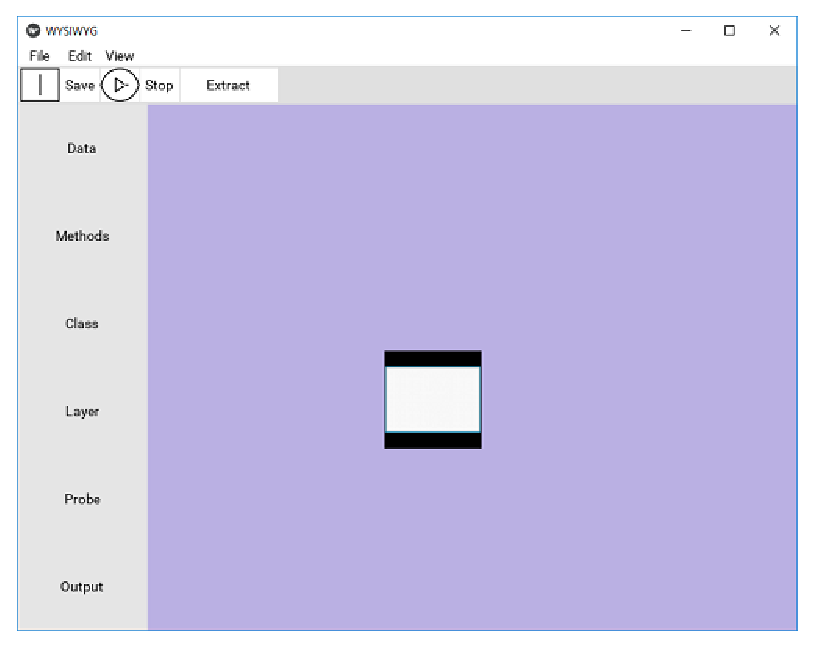
\includegraphics[width=\textwidth]{graphics/current_design.eps}
\caption{Current GUI}
\end{figure}
%------------------------------------------------------------------------------
\end{document}
